\documentclass[palatino]{apuntes}

\title{Infinite survival}
\author{Alejandro Moreno San Vidal \\ Pablo Pérez Manso}
\date{Videojuegos 2016}



\begin{document}
\pagestyle{plain}
\maketitle
\tableofcontents
\newpage

\chapter{Descripción general del proyecto}

\section{Introducción}
Este documento contiene las especificaciones de requisitos y el diseño del plan de trabajo del proyecto que se realizará por Alejandro Moreno San Vidal y Pablo Pérez Manso para la asignatura de Introducción a la Programación de Videojuegos.

\section{Descripción general del producto}
Este videojuego se desarrollará durante las prácticas de la asignatura, y su diseño y desarrollo se especifican en este documento. El videojuego será una combinación de las mecánicas que se observan en juegos tipo Endless Run, como son el caso de Zombie Tsunami o el popular Sonic, en la cual un personaje se mueve horizontalmente por la pantalla intentando recoger premios y evitando las cosas que le pueden matar.

\section{Funcionalidad}

El videojuego contará con las siguientes pantallas:
\begin{itemize}
    \item Pantalla de inicio
    \item Menú principal
    \item Ajustes
    \item Pantalla de juego
    \item Tablero de máximas puntuaciones
\end{itemize}

Cada pantalla tendrá las siguientes características y funcionalidades:
\begin{itemize}
    \item Pantalla de inicio
        \begin{itemize}
            \item Logo del juego
            \item Título del videojuego
            \item Botón para acceder al menú del juego
        \end{itemize}
    \item Menú principal
        \begin{itemize}
            \item Mostrará las principales acciones que se pueden realizar al empezar a jugar
            \item Botonera de opciones
                \begin{itemize}
                    \item Nueva partida
                    \item Ajustes
                    \item Puntuaciones
                \end{itemize}
        \end{itemize}
    \item Ajustes
        \begin{itemize}
            \item Ajustes de sonido
            \item Ajustes de usuario para las puntuaciones
        \end{itemize}
    \item Pantalla de juego
        \begin{itemize}
            \item Mostrará la partida que se está jugando actualmente
            \item Los elementos que contiene esta pantalla están determinados más adelante
        \end{itemize}
    \item Tablero de máximas puntuaciones
        \begin{itemize}
            \item Lista de las mejores puntuaciones (incluyendo multiples entradas de cada jugador)
            \item Lista de los mejores jugadores (una entrada por jugador con su mejor puntuación)
        \end{itemize}
\end{itemize}


\subsection{Acciones}
La pantalla del videojuego constará de un personaje que se mueve horizontalmente (de forma automática) y de izquierda a derecha y las acciones que podrá realizar son las siguientes:

\begin{itemize}
    \item \textbf{Saltar:} se producirá el salto para evitar enemigos o para salvar las caidas al vacío que puedan aparecer.
    \item \textbf{Agacharse:} en caso de que haya objetos a media altura, podrá optar no por saltarlos y esquivarlos agachándose.
    \item \textbf{Salto doble:} podrá realizarse esta acción si se desea coger objetos demasiado altos, salvar vacíos más largos o esquivar objetos muy extensos.
\end{itemize}


\subsection{Controles}
Los controles para las acciones descritas anteriormente serán:

\begin{itemize}
    \item \textbf{Saltar:}
        \begin{itemize}
            \item Un toque a la tecla de saltar hará un salto corto
            \item Una pulsación largar hará que el salto sea más largo (aunque no influirá en la altura del salto) 
        \end{itemize}
    \item \textbf{Agacharse:}
        \begin{itemize}
            \item Un toque hará que el personaje se agache durante un tiempo determinado
            \item Un toque mientras que el personaje está agachado, no sumará el tiempo, sino que será como si se hubiera agachado en ese momento
        \end{itemize}
    \item \textbf{Doble salto:}
        \begin{itemize}
            \item Si durante un salto se vuelve a presionar la tecla de salto, se producirá un doble salto
            \item Se puede hacer un doble salto tanto en saltos sencillos como en saltos largos
        \end{itemize}
\end{itemize}


\subsection{Estados}

\subsubsection{Estados del juego}
Los estados del juego serán los siguientes:

\begin{itemize}
    \item \textbf{Menú inicial}
        \begin{itemize}
            \item Es el estado inicial de nuestro juego
            \item Desde este menú se pueden acceder al resto de las pantallas: juegos, opciones, tablero...
        \end{itemize}
    \item \textbf{Pantalla de juego}
        \begin{itemize}
            \item En esta pantalla se producen todas las acciones del juego y su historia. Se muestra la pantalla de juego (véase 3.3 Interfaz de videojuego)
        \end{itemize}
    \item \textbf{Pausa}
        \begin{itemize}
            \item En la pausa se mostrará un menú en el que figuraran las siguientes opciones
                \begin{itemize}
                    \item Contadores del estado actual de la partida
                    \item Siguiente marca a batir actualmente
                    \item Botonera para diferentes acciones 
                         \begin{itemize}
                            \item Volver al juego
                            \item Reiniciar partida
                            \item Ir al menú principal
                        \end{itemize}
                \end{itemize}
        \end{itemize}
    \item \textbf{Death}
        \begin{itemize}
            \item Se mostrará el resultado final de la partida
            \item Botonera para diferentes acciones
                \begin{itemize}
                    \item Reiniciar la partida
                    \item Volver al menú principal
                \end{itemize}
        \end{itemize}
\end{itemize}


\subsubsection{Estados del personaje}
El personaje podrá encontrarse en los siguientes estados

\begin{itemize}
    \item Corriendo
    \begin{itemize}
        \item Es el estado que se mantendrá la mayor parte del tiempo
        \item Desde este estado se puede llegar a cualquiera de los otros
    \end{itemize}
    \item Saltando
    \begin{itemize}
        \item Se entra en este estado cuando se presiona la tecla de saltar
        \item Se sale automáticamente al tocar un objeto o al volver a pulsar el botón de salto (en el caso de un salto sencillo)
    \end{itemize}
    \item Agachado
    \begin{itemize}
        \item Sólo se podrá entrar a este estado desde el estado de corriendo
        \item Tendrá una duración predeterminada
        \item Para pronlogar su duración se podrá volver a presionar la tecla de agacharse mientras se está en este estado
    \end{itemize}
    \item Muerto
    \begin{itemize}
        \item Se llega a través del resto de los estados
        \item Indicará que se ha acabado la partida y que se tendrá que lanzar la pantalla de fin de partida
    \end{itemize}
\end{itemize}


\subsection{Mecánica del juego}
En esta sección se intentará dar una aproximación de cómo se pretende que sea el uso del juego. No debe tomarse como un manual del mismo, ya que es posible que surjan cambios durante el desarrollo del proyecto, ni como descripción de controles y acciones (secciones anteriores) ni como su intefaz gráfica (secciones venideras).

La mecánica del juego consistirá en una carrera continua automática sobre la que el jugador no tendrá ninguna capacidad de cambiar. Éste deberá utilizar los comandos explicados anteriormente para esquivar los problemas que se le puedan ir planteando a lo largo del juego. Así mismo, el jugador deberá cubrir la distancia más larga para conseguir una puntuación mayor así como recoger objetos que le puedan ayudar durante el juego.

La dificultad del juego residirá en que durante la carrera, se irán poniendo diferentes travas para que la dificultad vaya en aumento:

\begin{itemize}
    \item La \textbf{velocidad aumentará} de modo que los nuevos enemigos y la pantalla aparecerá cada vez más rápido dando menos tiempo al jugador a reaccionar ante estos imprevistos, siendo los reflejos clave para poder continuar jugando.
    \item La \textbf{densidad de obstáculos aumentará}, de modo que cada vez haya más enemigos y cada vez más juntos siendo necesario aplicar saltos más complicados o tener que calcular de una forma más precisa las caidas de los saltos.
\end{itemize}

Además durante el juego se le ofrecerán al jugador mejoras que podrá ir cogiendo durante el juego, tales como powerups que le harán más fácil la partida o le añadirán características interesantes durante el desarrollo del juego.

El juego terminará si la vida del personaje tras chocharse con objetos llega a cero, siendo esta recuperable con diferentes objetos del juego. Además también se terminará cuando la pantalla coma al jugador, es decir, que cuando un objeto se interponga en el avance del jugador y éste desaparezca por el lado izquierdo de la pantalla.


\section{Dominio}
Aunque no está categorizado como un tipo de juego, "Enless Run" es el mejor término que lo define. Un personaje corre sin parar y sin fin por una linea horizontal siendo el objetivo del juego evitar todos los enemigos posibles y conseguir todas las mejoras ofrecidas.


\section {Entorno y herramientas de desarrollo}
El juego va a ser desarrollado bajo la plataforma Phaser.io. Esta plataforma ha de ser trabajada con el lenguaje de programación Javascript y mediante un servidor web. Las herramientas que se utilizarán serán las siguientes:

\begin{itemize}
	\item \textbf{Linux:} se utilizará un entorno de desarrollo linux junto con las herramientas de texlive para la generación de documentos mediante el lenguaje \LaTeX.
	\item \textbf{Git y Github:} como control de versiones el proyecto se sostendrá sobre git, ya que permite una estructura descentralizada de desarrollo en la que se puede editar en concurrencia. Además, para mantener un backup online y una forma de sincornizar código, se utilizará la plataforma github, así como registro online del trabajo que vamos desarrollando.
	\item \textbf{Adobe Photoshop e Illustrator:} con la intención de desarrollar los diferentes aspectos gráficos del juego se utilizarán estos programas con el fin de hacer correcciones o crear nuevos gráficos para el juego.
	\item \textbf{Adobe Audition:} edición de los diferentes temas musicales y efectos sonoros del juego.
	\item \textbf{Sublime Text, Brackets y/o vim:} ya que el lenguaje que se utilizará no tiene ningún entorno de desarrollo establecido y que ofrezca ventajas significativas se utilizará un editor de código sencillo para el desarrollo del juego.
	\item \textbf{Brackets y XAMPP:} dada la necesidad de necesitar un servidor web que se encargue de los diferentes aspectos del juego, éstos serán los escogidos para la realización de las pruebas.
\end{itemize}

Como la mayoría de estos programas son gratuitos o se disponen de las diferentes licencias necesarias para el desarrollo de todo el sistema, el coste en herramientas del desarrollo del proyecto será gratuito.


\section{Descripción del hardware}
Para el desarrollo de todo lo anteriormente descrito y el uso de las herramientas planteadas en la sección anterior se necesitarán los siguiente requisitos hardware:

\begin{itemize}
	\item Ordenador con un dual boot o una máquina virtual en el que estén preinstalados una distribución Linux y una versión de Windows superior a la 7.
	\item El ordenador deberá tener ratón y teclado, no sólo para trabajar, sino también para poder realizar las pruebas del juego.
	\item Un gamepad con el fin de probar el videojuego, ya que éste, también será compatible con este tipo de mandos.
\end{itemize}


\section{Equipo y lugar de trabajo}
El equipo constará de dos personas que conforman la pareja de prácticas y que compartirán todas las tareas que se especificarán en la sección 2.

El lugar de trabajo, será mayoritariamente los laboratorios de la Escuela Politécnica Superior de la Universidad Autónoma de Madrid, ya que todos disponen en su mayoría de los requisitos de software y hardware descritos anteriormente. Así mismo, también se plantea que, de no poderse utilizar los laboratorios por horarios o necesidades varias, se hará uso de máquinas personales que podrán ser utilizadas en el lugar más conveniente.


\section{Recursos adicionales}
En lo referente a recursos que todavía no se han mencionado se preveen lo siguientes:

\begin{itemize}
	\item \textbf{Sprites:} personajes y diferentes objetos serán cogidos de presets ya creados por otros usuarios de internet.
	\item \textbf{Menús y fondos:} al igual que los sprites se realizarán búsquedas por internet o se procederá a la generación de los mismos.
	\item \textbf{Música y efectos sonoros:} se recurriran a bibliotecas de sonido online para poder desarrollar todos los sonidos del juego. De no ser posible, se procedería a la grabación de todo el material que fuera necesario.
	\item \textbf{Tipografías:} las diferentes tipografías que se utilizarán en el juego se extraerán de plataformas online como Google Fonts.
\end{itemize}

Todo este material se utilizará siendo la licencia de los mismos compatibles con la licencia que establezca para el proyecto.










\chapter{Gestión del Proyecto}
En esta sección se mostrarán los aspectos de la planificación del proyecto, desde tareas, plazos de entrega y la línea temporal, hasta los entregables y su contenido.

\section{Tareas a realizar}
El gráfico con las tareas del desarrollo del proyecto y su plan temporal se encuentran en los anexos de este documento. Si se necesita más información se puede recurrir al capítulo 3 de este documento en el que se epsecifica más del Análisis y Diseño.

\section{Entregables}

Se plantea el diseño del videojuego en tres entregas, incluyendo la que se realiza con este documento. Las entregas se detallan a continuación:

\begin{itemize}
	\item \textbf{Documento de diseño previo del videojuego:} recoge las funcionaledades y aspectos generales del videojuego a realizar, todo incluido en el presente documento. Su entrega se prevee al principio del desarrollo.
	\item \textbf{Prototipo del proyecto:} se entregará un prototipo funcional del proyecto en el que se pueda probar una primera versión del videojuego y en el que se podrán apreciar los diferentes cambios que se han realizado respecto de este documento. Todos esos cambios se especificarán en otro documento. Se prevee su entrega a la mitad del desarrollo.
	\item \textbf{Entrega final:} se entregará una versión del desarrollo completamente operativa y con todas las funcionalidades previamente descritas ya implementadas. Así mismo se entregará una memoria de todo el desarrollo del proyecto y un manual de uso del juego en el que se expondrán todos los aspectos relevantes del juego. Su entrega se preve con la finalización del plazo.
\end{itemize}










\chapter{Análisis y diseño}
Procederemos con los temas referentes a la planificación del proyecto, incluyendo el ciclo de vida del software, planteamiento de diseño a seguir y los diagramas que nos permitirán desarrollar e implementar todas las funcionalidades y aspectos descritos en el capítulo 1.

\section{Modelo de ciclo de vida}

Para el ciclo de vida de nuestro proyecto se tomará un diseño basado en cascada con realimentación, de modo que nos permite rápidamente volver a la fase anterior para corregir los errores que se pudieran haber cometido. Constará de las siguientes fases:

\begin{enumerate}
	\item \textbf{Análisis:} se analizan y se definen todas las funcionalidades y los requisitos que necesitará el proyecto, de modo que se pueda tener claro en la fase de diseño qué debería recoger.
	\item \textbf{Diseño:} se escoge cual es el mejor método para llevar a cabo el proyecto en base a las especificaciones que se observaron en la fase de análisis y se plasman en una serie de documentos. Esto incluirá  la planificación temporal, funcionalidades y forma de implementarlas y todos los demás aspectos del proyecto.
	\item \textbf{Implmementación:} se comenzará con el desarrollo de toda la parte técnica del proyecto, de modo que sea coherente con todos los detalles que se planificaron previamente en la fase de diseño. Así mismo se podrán generar prototipos de todo el proyecto o de partes de él para que puedan pasar a la siguiente fase.
	\item \textbf{Pruebas:} una buena parte del desarrollo es probar que todo lo anteriormente implementado funcione como se especificó en la parte de diseño. En esta fase se podrían incluso mostrar diversos prototipos al cliente final para que pueda observar el estado del proyecto. En caso de un error detectado se notificará y se devolverá a la fase de implementación o diseño, dependiendo del error.
	\item \textbf{Entregas:} una vez que los prototipos que ya se planificaron en la fase de diseño, pasen la fase de pruebas se realiarán diferentes entregas de material al cliente para que se pueda ir evaluando el trabajo que se está desarrollando y que éste localice diferentes errores que como cliente no desee o no quedaran claras en la fase previa al análisis.
	\item \textbf{Entrega del producto y mantenimiento:} una vez terminada toda las fases de desarrollo del proyecto se procederá con la entrega del mismo al cliente, y se mantendrá un periodo de mantenimiento en el que el cliente podrá notificar posibles errores o mejoras que se podrán implementar.
\end{enumerate}

\begin{figure}[hbtp]
    \centering
    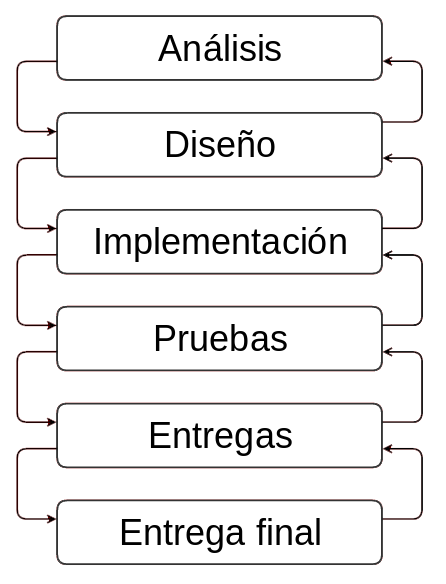
\includegraphics[width=0.4\textwidth]{img/cascada.png}
    \caption{Cascada con realimentación}
    \label{fig:cascadarealimentacion}
\end{figure}





\section{Diseño}

Para poder proceder correctamente con la implementación del proyecto es necesario realizar un diseño modular de todo el código del videojuego. Se diseñarán las clases del código a implmentar que darán forma a los elementos del videojuego.

En esta sección se especificarán las implementaciones de la mayoría de los elementos descritos en la primera sección del documento, por lo que es recomendable que se consulte como referencia si en alguna parte de esta sección se tienen dudas.

Todo el videojuego será controlado por una clase Juego que contendrá todo el resto de los elementos del sistema. Esta contendrá al jugador, powerups(objetos que el jugador podrá obtener), los enemigos (elementos perjudiciales para el jugador) y el mapa.

\begin{itemize}
	\item El jugador tendrá entidad única para el mismo debido a su diferencia con el resto de instancias del juego. Además se le podrán cambiar diferentes aspectos de su física natural en base a los objetos que pueda ir recogiendo.
	\item Los powerups y los enemigos se proponen como objetos distintos ya que a la hora de afectar al jugador por igual se analizarán primero unos antes que otros.
	\item El mapa se irá generando automáticamente o cargando de ficheros externos para poder ir dibujando todo el sistema de juego.
\end{itemize}

Además se realizarán clases e interfaces que resuelvan las diferentes acciones que puedan ocurrir en el juego, como las colisiones entre objetos, los controles por parte de los diferentes dispositivos, así como las conexiones con el servidor de puntuaciones.


\section{Interfaz del videojuego}
La parte del videojuego que el cliente termina viendo es una de las más importantes a la hora del desarrollo del videojuego, por lo que en esta sección se pretende dar una idea de la composición de la interfaz de ususario. Se mostrará un ejemplo de otro juego con una interfaz similar a la que se quiere implementar.

Los elementos que se mostrarán son los que siguen:
\begin{itemize}
	\item \textbf{Fondo:} se mostrará un fondo que refleje la situación del personaje dependiendo del traje que lleve en cada momento, de forma que pueda hacer que el usuario tenga una inmersión en el videojuego mayor.
	\item \textbf{Personaje:} el personaje principal será una imagen que por norma general se encontrará en el centro del escenario. Dependiendo de diferentes mejoras del juego se podrá cambiar la imagen del mismo para poder reflejar mejor las mejoras que pueda haber conseguido.
	\item \textbf{Barra superior:} en esta se mostrarán los principales indicadores del juego para que el jugador las pueda ver:
		\begin{itemize}
			\item \textbf{Distancia:} distancia (puntuación) recorrida por el personaje en la partida
			\item \textbf{Vida:} un indicador en el que se diga la vida que le queda al jugador
		\end{itemize}
	\item \textbf{Objetos recogidos:} se pueden ir recogiendo objetos por el juego que luego se podrán usar con diferentes acciones. Para poder conocer que objetos tienes disponibles se dispondrán en una tira en un lado de la pantalla.
	
	\item \textbf{Enemigos y mejoras:} durante la carrera irán apareciendo por el escenario distintos enemigos, obstáculos y objetos de mejora que el personaje tendrá que coger o esquivar.
\end{itemize}

La interfaz sería parecida a la siguiente:

\begin{figure}[hbtp]
    \centering
    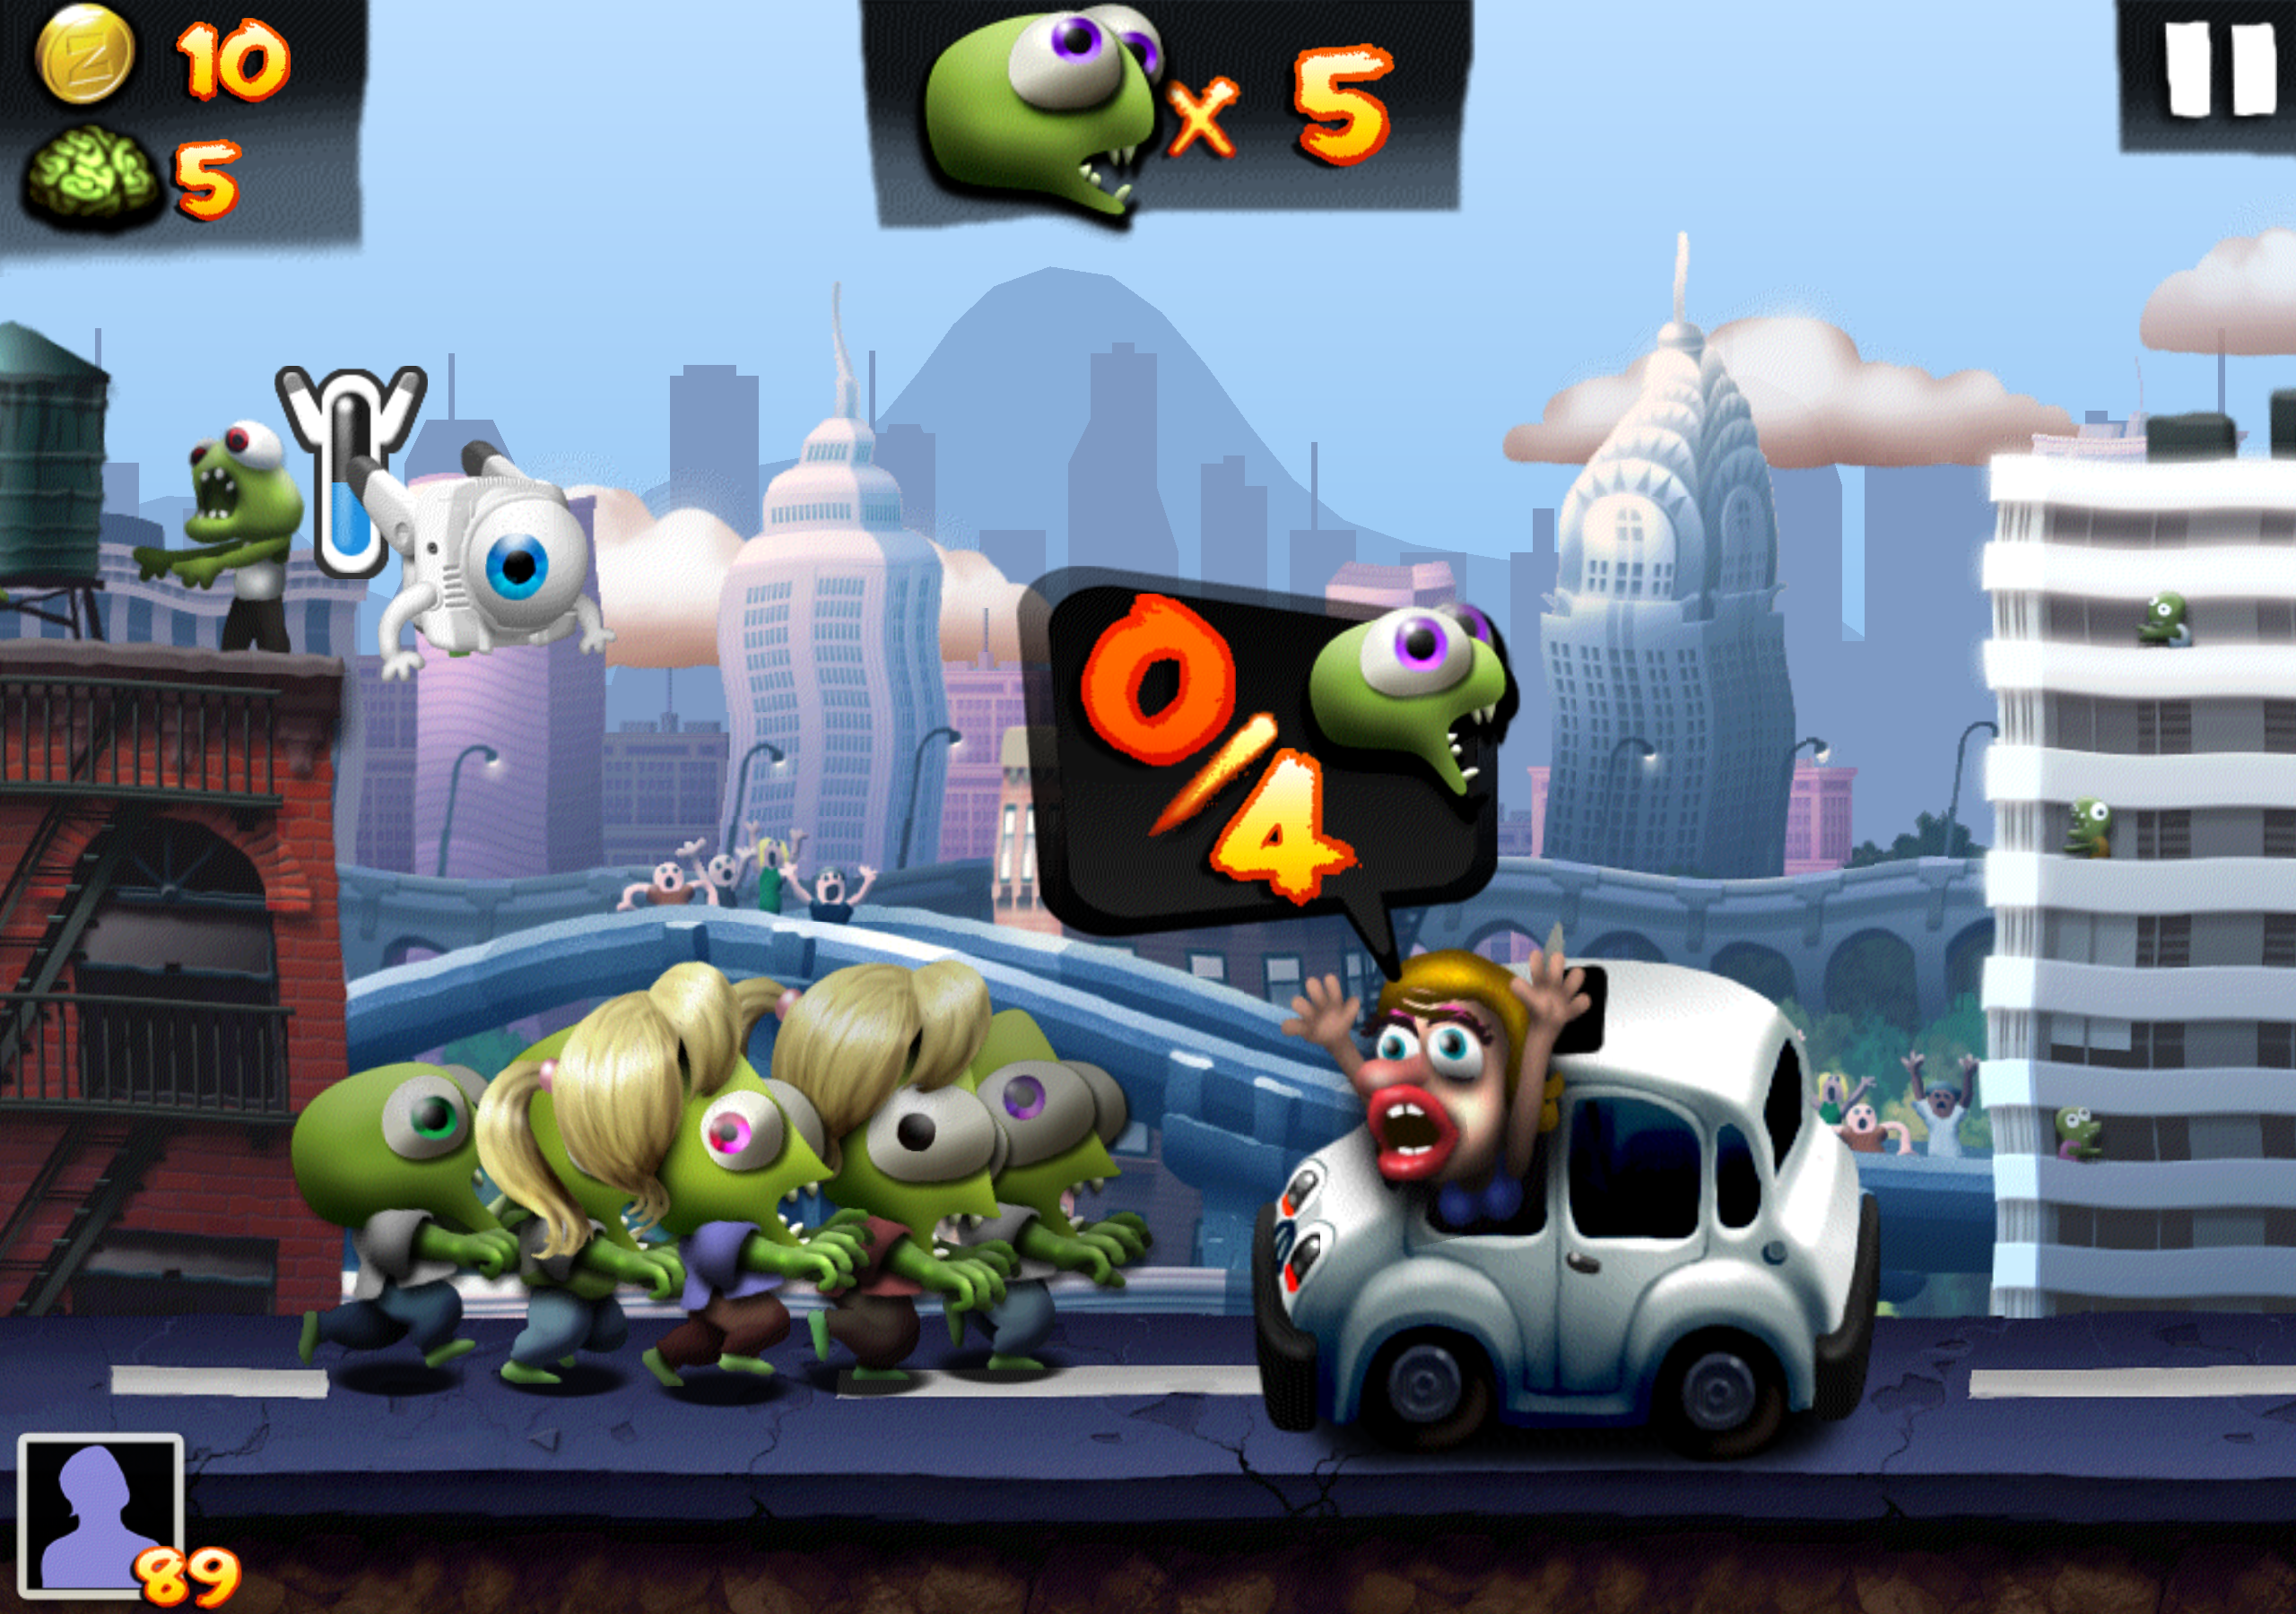
\includegraphics[width=0.8\textwidth]{img/captura_zombies.png}
    \caption{Interfaz similar a la descrita}
    \label{fig:interfazzombie}
\end{figure}


\chapter{Implementación}
Para facilitar la creación y la relación entre las clases definidas en la fase de diseño, se ha considerado el uso de patrones de diseño. Además se tratará de que el diseño sea lo más modular posible.

Se van a usar dos tipos de patrones: de creación, para ayudar a crear los nuevos objetos en tiempo de ejecución y estructurales, para mejorar la organización del código.

Para los patrones de creación se considera el siguiente:
\begin{itemize}
	\item \textbf{Singleton}: nos permite que algunas de las clases solo puedan ser creadas una vez de modo que su control es mucho más fácil por el resto de las clases. Sería los casos del juego o del personaje.
\end{itemize}

En cuanto a los patrones estructurales se considera el siguiente:
\begin{itemize}
	\item \textbf{Modelo Vista Controlador:} ayuda a organizar la lógica interna de modo que se separa por completo la parte de la interfaz de los datos que se manejan. De este modo se crea más independencia entre cada uno de los módulos pudiendo cambiar cada uno de ellos sin necesidad de cambiar el otro.
\end{itemize}

En lo que respecta a las fases de la implementación se consideran tres fases:

\begin{itemize}
	\item \textbf{Lógica:} nos referimos a la parte de toda la codificación de la parte lógica del videojuego, personajes, objetos, pantalla...
	\item \textbf{Gráficos:} búsqueda de posibles materiales gráficos para la temática del juego y su adaptación a las necesidades del proyecto.
	\item \textbf{Interfaz:} una vez finalizada la parte de gráficos, construcción de la interfaz basada en esos gráficos y su unión con la lógica del juego.
\end{itemize}


\chapter{Pruebas}
Para una correcta integración de todas las partes del proyecto, se deben realizar pruebas para que una vez que se realice la integración no haya ningún problema.

\begin{itemize}
	\item \textbf{Lógica:} se hará una comprobación de que todas las clases tienen un funcionamiento correcto y más tarde se probará sun funcionalidad conjunta. De este modo nos aseguraremos que esta parte funciona de una forma correcta para que al añadir la parte de interfaz se minimicen los errores.
	\item \textbf{Gráficos:} se cargarán todos los sprites, dibujos, imágenes y sonidos sobre una instancia de phaser nueva para comprobar que funcionan de un modo de adecuado con la plataforma al ser cargados.
	\item \textbf{Interfaz:} se probarán la cohesión que tienen la creación de la parte gráfica con la lógica del videojuego. Se comproborará que la comunicación entre la lógica y la interfaz se produce de manera correcta, viéndose en la pantalla lo que corresponde por la parte del backend. Además se deberán hacer diferentes pruebas de velocidad del sistema para corregir errores de implementación a la hora de pintar la interfaz.
\end{itemize}

Cabe destacar, que debido a la complejidad de algunos de los componentes de la parte lógica, su correcto funcionamiento será comprobado mediante su salida por la interfaz, de modo que se comprueba a la vez parte de la lógica y parte de la interfaz.


\newpage
%% Apendices (ejercicios, examenes)
\appendix
\chapter{Planificación temporal}

\begin{figure}[hbtp]
    \centering
    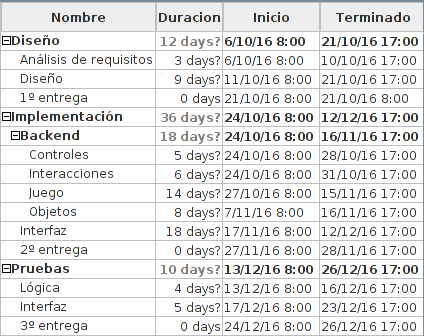
\includegraphics[width=0.8\textwidth]{img/tabla_tiempos.png}
    \caption{Tiempos de cada tarea}
    \label{fig:tiempostarea}
\end{figure}

\newpage

\begin{figure}[hbtp]
    \centering
    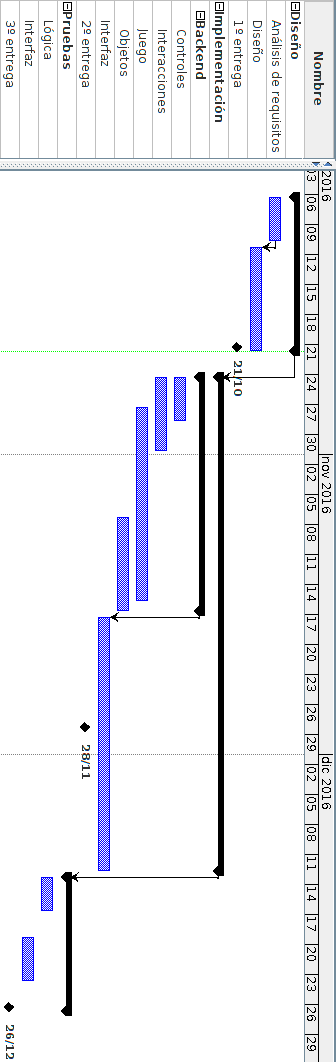
\includegraphics[width=0.5\textwidth]{img/gant_completo.png}
    \caption{Diagrama de Gant}
    \label{fig:diagramagant}
\end{figure}

\end{document}